\begin{figure} 
	\centering
	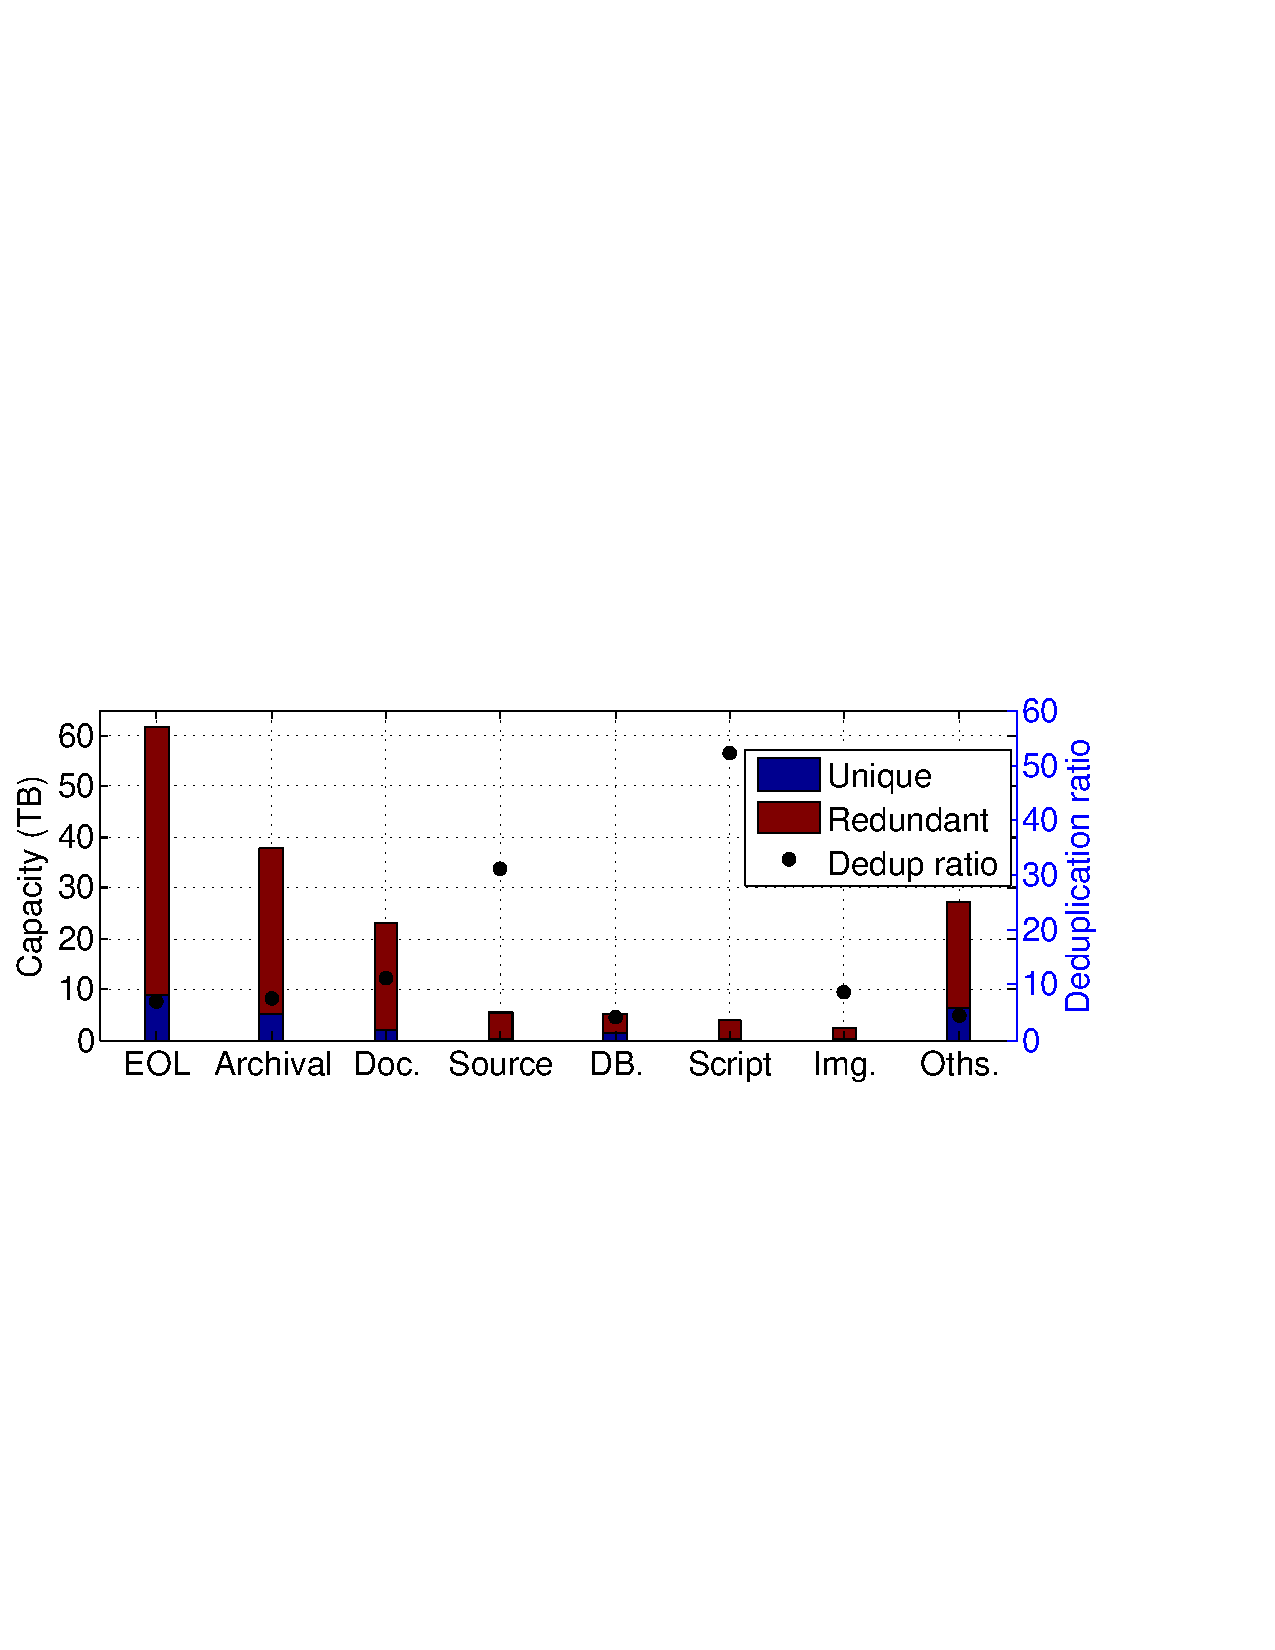
\includegraphics[width=0.45\textwidth]{graphs/dedup-overall} 
	\caption{Deduplication ratio for seven file classes---EOL, archival, documents, source code, database, scripts, images---and other files.
	Blue bar represents the capacity after removing redundant file duplicates. White bar indicates how much redundant data is removed after deduplication. The dot shows the deduplication ratio in terms of capacity.
%
\VT{Can we stretch X axis to column width to have more space for X-axis labels?}\NZ{addressed}
%
\VT{Explain what blue and red bars mean here, as well as dots. Explain
if dedup ratio is in terms of capacity or file counts.}\NZ{addressed}
%
} 
	\label{fig:dedup-overall} 
\end{figure}


